\documentclass[twoside]{book}

% Packages required by doxygen
\usepackage{calc}
\usepackage{doxygen}
\usepackage{graphicx}
\usepackage[utf8]{inputenc}
\usepackage{makeidx}
\usepackage{multicol}
\usepackage{multirow}
\usepackage{textcomp}
\usepackage[table]{xcolor}

% Font selection
\usepackage[T1]{fontenc}
\usepackage{mathptmx}
\usepackage[scaled=.90]{helvet}
\usepackage{courier}
\usepackage{amssymb}
\usepackage{sectsty}
\renewcommand{\familydefault}{\sfdefault}
\allsectionsfont{%
  \fontseries{bc}\selectfont%
  \color{darkgray}%
}
\renewcommand{\DoxyLabelFont}{%
  \fontseries{bc}\selectfont%
  \color{darkgray}%
}

% Page & text layout
\usepackage{geometry}
\geometry{%
  a4paper,%
  top=2.5cm,%
  bottom=2.5cm,%
  left=2.5cm,%
  right=2.5cm%
}
\tolerance=750
\hfuzz=15pt
\hbadness=750
\setlength{\emergencystretch}{15pt}
\setlength{\parindent}{0cm}
\setlength{\parskip}{0.2cm}
\makeatletter
\renewcommand{\paragraph}{%
  \@startsection{paragraph}{4}{0ex}{-1.0ex}{1.0ex}{%
    \normalfont\normalsize\bfseries\SS@parafont%
  }%
}
\renewcommand{\subparagraph}{%
  \@startsection{subparagraph}{5}{0ex}{-1.0ex}{1.0ex}{%
    \normalfont\normalsize\bfseries\SS@subparafont%
  }%
}
\makeatother

% Headers & footers
\usepackage{fancyhdr}
\pagestyle{fancyplain}
\fancyhead[LE]{\fancyplain{}{\bfseries\thepage}}
\fancyhead[CE]{\fancyplain{}{}}
\fancyhead[RE]{\fancyplain{}{\bfseries\leftmark}}
\fancyhead[LO]{\fancyplain{}{\bfseries\rightmark}}
\fancyhead[CO]{\fancyplain{}{}}
\fancyhead[RO]{\fancyplain{}{\bfseries\thepage}}
\fancyfoot[LE]{\fancyplain{}{}}
\fancyfoot[CE]{\fancyplain{}{}}
\fancyfoot[RE]{\fancyplain{}{\bfseries\scriptsize Generated on Thu Sep 17 2015 22\-:52\-:12 for G\-H\-O\-S\-T C\# by Doxygen }}
\fancyfoot[LO]{\fancyplain{}{\bfseries\scriptsize Generated on Thu Sep 17 2015 22\-:52\-:12 for G\-H\-O\-S\-T C\# by Doxygen }}
\fancyfoot[CO]{\fancyplain{}{}}
\fancyfoot[RO]{\fancyplain{}{}}
\renewcommand{\footrulewidth}{0.4pt}
\renewcommand{\chaptermark}[1]{%
  \markboth{#1}{}%
}
\renewcommand{\sectionmark}[1]{%
  \markright{\thesection\ #1}%
}

% Indices & bibliography
\usepackage{natbib}
\usepackage[titles]{tocloft}
\setcounter{tocdepth}{3}
\setcounter{secnumdepth}{5}
\makeindex

% Hyperlinks (required, but should be loaded last)
\usepackage{ifpdf}
\ifpdf
  \usepackage[pdftex,pagebackref=true]{hyperref}
\else
  \usepackage[ps2pdf,pagebackref=true]{hyperref}
\fi
\hypersetup{%
  colorlinks=true,%
  linkcolor=blue,%
  citecolor=blue,%
  unicode%
}

% Custom commands
\newcommand{\clearemptydoublepage}{%
  \newpage{\pagestyle{empty}\cleardoublepage}%
}


%===== C O N T E N T S =====

\begin{document}

% Titlepage & ToC
\hypersetup{pageanchor=false}
\pagenumbering{roman}
\begin{titlepage}
\vspace*{7cm}
\begin{center}%
{\Large G\-H\-O\-S\-T C\# }\\
\vspace*{1cm}
{\large Generated by Doxygen 1.8.6}\\
\vspace*{0.5cm}
{\small Thu Sep 17 2015 22:52:12}\\
\end{center}
\end{titlepage}
\clearemptydoublepage
\tableofcontents
\clearemptydoublepage
\pagenumbering{arabic}
\hypersetup{pageanchor=true}

%--- Begin generated contents ---
\chapter{Namespace Index}
\section{Namespace List}
Here is a list of all documented namespaces with brief descriptions\-:\begin{DoxyCompactList}
\item\contentsline{section}{\hyperlink{namespaceghost}{ghost} }{\pageref{namespaceghost}}{}
\end{DoxyCompactList}

\chapter{Hierarchical Index}
\section{Class Hierarchy}
This inheritance list is sorted roughly, but not completely, alphabetically\-:\begin{DoxyCompactList}
\item \contentsline{section}{ghost.\-Constraint$<$ Type\-Set\-Variables, Type\-Variable $>$}{\pageref{classghost_1_1Constraint_3_01TypeSetVariables_00_01TypeVariable_01_4}}{}
\item I\-Cloneable\begin{DoxyCompactList}
\item \contentsline{section}{ghost.\-Domain}{\pageref{classghost_1_1Domain}}{}
\end{DoxyCompactList}
\item \contentsline{section}{ghost.\-Objective$<$ Type\-Set\-Variables, Type\-Variable $>$}{\pageref{classghost_1_1Objective_3_01TypeSetVariables_00_01TypeVariable_01_4}}{}
\begin{DoxyCompactList}
\item \contentsline{section}{ghost.\-Null\-Objective$<$ Type\-Set\-Variables, Type\-Variable $>$}{\pageref{classghost_1_1NullObjective_3_01TypeSetVariables_00_01TypeVariable_01_4}}{}
\end{DoxyCompactList}
\item \contentsline{section}{ghost.\-Set\-Variables$<$ Type\-Variable $>$}{\pageref{classghost_1_1SetVariables_3_01TypeVariable_01_4}}{}
\item \contentsline{section}{ghost.\-Solver$<$ Type\-Variable, Type\-Set\-Variables, Type\-Constraint $>$}{\pageref{classghost_1_1Solver_3_01TypeVariable_00_01TypeSetVariables_00_01TypeConstraint_01_4}}{}
\item \contentsline{section}{ghost.\-Variable}{\pageref{classghost_1_1Variable}}{}
\end{DoxyCompactList}

\chapter{Class Index}
\section{Class List}
Here are the classes, structs, unions and interfaces with brief descriptions\-:\begin{DoxyCompactList}
\item\contentsline{section}{\hyperlink{classghost_1_1Constraint_3_01TypeSetVariables_00_01TypeVariable_01_4}{ghost.\-Constraint$<$ Type\-Set\-Variables, Type\-Variable $>$} }{\pageref{classghost_1_1Constraint_3_01TypeSetVariables_00_01TypeVariable_01_4}}{}
\item\contentsline{section}{\hyperlink{classghost_1_1Domain}{ghost.\-Domain} }{\pageref{classghost_1_1Domain}}{}
\item\contentsline{section}{\hyperlink{classghost_1_1NullObjective_3_01TypeSetVariables_00_01TypeVariable_01_4}{ghost.\-Null\-Objective$<$ Type\-Set\-Variables, Type\-Variable $>$} }{\pageref{classghost_1_1NullObjective_3_01TypeSetVariables_00_01TypeVariable_01_4}}{}
\item\contentsline{section}{\hyperlink{classghost_1_1Objective_3_01TypeSetVariables_00_01TypeVariable_01_4}{ghost.\-Objective$<$ Type\-Set\-Variables, Type\-Variable $>$} }{\pageref{classghost_1_1Objective_3_01TypeSetVariables_00_01TypeVariable_01_4}}{}
\item\contentsline{section}{\hyperlink{classghost_1_1SetVariables_3_01TypeVariable_01_4}{ghost.\-Set\-Variables$<$ Type\-Variable $>$} }{\pageref{classghost_1_1SetVariables_3_01TypeVariable_01_4}}{}
\item\contentsline{section}{\hyperlink{classghost_1_1Solver_3_01TypeVariable_00_01TypeSetVariables_00_01TypeConstraint_01_4}{ghost.\-Solver$<$ Type\-Variable, Type\-Set\-Variables, Type\-Constraint $>$} }{\pageref{classghost_1_1Solver_3_01TypeVariable_00_01TypeSetVariables_00_01TypeConstraint_01_4}}{}
\item\contentsline{section}{\hyperlink{classghost_1_1Variable}{ghost.\-Variable} }{\pageref{classghost_1_1Variable}}{}
\end{DoxyCompactList}

\chapter{Namespace Documentation}
\hypertarget{namespaceghost}{\section{Package ghost}
\label{namespaceghost}\index{ghost@{ghost}}
}
\subsection*{Classes}
\begin{DoxyCompactItemize}
\item 
class \hyperlink{classghost_1_1Constraint_3_01TypeSetVariables_00_01TypeVariable_01_4}{Constraint$<$ Type\-Set\-Variables, Type\-Variable $>$}
\item 
class \hyperlink{classghost_1_1Domain}{Domain}
\item 
class \hyperlink{classghost_1_1Objective_3_01TypeSetVariables_00_01TypeVariable_01_4}{Objective$<$ Type\-Set\-Variables, Type\-Variable $>$}
\item 
class \hyperlink{classghost_1_1NullObjective_3_01TypeSetVariables_00_01TypeVariable_01_4}{Null\-Objective$<$ Type\-Set\-Variables, Type\-Variable $>$}
\item 
class \hyperlink{classghost_1_1SetVariables_3_01TypeVariable_01_4}{Set\-Variables$<$ Type\-Variable $>$}
\item 
class \hyperlink{classghost_1_1Solver_3_01TypeVariable_00_01TypeSetVariables_00_01TypeConstraint_01_4}{Solver$<$ Type\-Variable, Type\-Set\-Variables, Type\-Constraint $>$}
\item 
class \hyperlink{classghost_1_1Variable}{Variable}
\end{DoxyCompactItemize}

\chapter{Class Documentation}
\hypertarget{classghost_1_1Constraint_3_01TypeSetVariables_00_01TypeVariable_01_4}{\section{ghost.\-Constraint$<$ Type\-Set\-Variables, Type\-Variable $>$ Class Template Reference}
\label{classghost_1_1Constraint_3_01TypeSetVariables_00_01TypeVariable_01_4}\index{ghost.\-Constraint$<$ Type\-Set\-Variables, Type\-Variable $>$@{ghost.\-Constraint$<$ Type\-Set\-Variables, Type\-Variable $>$}}
}
\subsection*{Public Member Functions}
\begin{DoxyCompactItemize}
\item 
\hypertarget{classghost_1_1Constraint_3_01TypeSetVariables_00_01TypeVariable_01_4_ac4aba3edfc75f14a974cf45c9a4fbe0d}{abstract double {\bfseries Cost} (double\mbox{[}$\,$\mbox{]} variable\-Cost)}\label{classghost_1_1Constraint_3_01TypeSetVariables_00_01TypeVariable_01_4_ac4aba3edfc75f14a974cf45c9a4fbe0d}

\item 
\hypertarget{classghost_1_1Constraint_3_01TypeSetVariables_00_01TypeVariable_01_4_a5ac6b63a92e54e8812bcdd414763d852}{abstract Dictionary$<$ int, double $>$ {\bfseries Simulate\-Cost} (int current\-Variable\-Index, Dictionary$<$ int, double\mbox{[}$\,$\mbox{]} $>$ variable\-Sim\-Cost)}\label{classghost_1_1Constraint_3_01TypeSetVariables_00_01TypeVariable_01_4_a5ac6b63a92e54e8812bcdd414763d852}

\end{DoxyCompactItemize}
\subsection*{Protected Member Functions}
\begin{DoxyCompactItemize}
\item 
\hypertarget{classghost_1_1Constraint_3_01TypeSetVariables_00_01TypeVariable_01_4_af5f29309c2d8a5874f8e89d9237ae156}{{\bfseries Constraint} (Type\-Set\-Variables variables)}\label{classghost_1_1Constraint_3_01TypeSetVariables_00_01TypeVariable_01_4_af5f29309c2d8a5874f8e89d9237ae156}

\end{DoxyCompactItemize}
\subsection*{Properties}
\begin{DoxyCompactItemize}
\item 
\hypertarget{classghost_1_1Constraint_3_01TypeSetVariables_00_01TypeVariable_01_4_a22327beeea2a2d774f85477a9fdd7b55}{Type\-Set\-Variables {\bfseries Variables}\hspace{0.3cm}{\ttfamily  \mbox{[}get, set\mbox{]}}}\label{classghost_1_1Constraint_3_01TypeSetVariables_00_01TypeVariable_01_4_a22327beeea2a2d774f85477a9fdd7b55}

\end{DoxyCompactItemize}


The documentation for this class was generated from the following file\-:\begin{DoxyCompactItemize}
\item 
Ghost/src/Constraint.\-cs\end{DoxyCompactItemize}

\hypertarget{classghost_1_1Domain}{\section{ghost.\-Domain Class Reference}
\label{classghost_1_1Domain}\index{ghost.\-Domain@{ghost.\-Domain}}
}
Inheritance diagram for ghost.\-Domain\-:\begin{figure}[H]
\begin{center}
\leavevmode
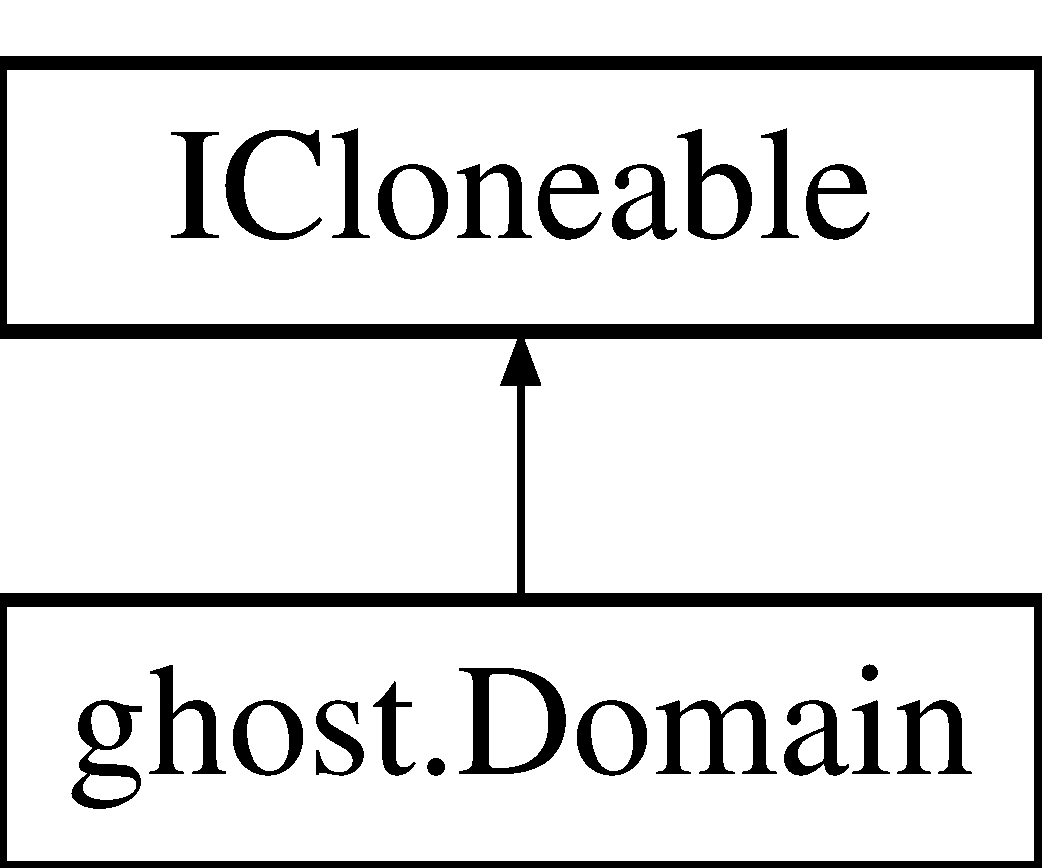
\includegraphics[height=2.000000cm]{classghost_1_1Domain}
\end{center}
\end{figure}
\subsection*{Public Member Functions}
\begin{DoxyCompactItemize}
\item 
\hyperlink{classghost_1_1Domain_a62af4592a700051d017678189d1f9d2a}{Domain} (int outside\-Scope=-\/1)
\item 
\hyperlink{classghost_1_1Domain_ad73e5c9b5f2044affc5c45fe09f39577}{Domain} (List$<$ int $>$ domain, int outside\-Scope)
\item 
\hyperlink{classghost_1_1Domain_ab3bd027fd023c60ba95ace0108a1c2f7}{Domain} (int size, int start\-Value)
\item 
\hypertarget{classghost_1_1Domain_a4cac9f43b65f302a15cf6cef40eae625}{object {\bfseries Clone} ()}\label{classghost_1_1Domain_a4cac9f43b65f302a15cf6cef40eae625}

\item 
bool \hyperlink{classghost_1_1Domain_a19610b0d083f6a47eeb867fbcf8c0522}{Is\-Initialized} ()
\item 
void \hyperlink{classghost_1_1Domain_a732f5cc39dba50b1abbfc37664a3bbb7}{Reset\-To\-Initial} ()
\item 
bool \hyperlink{classghost_1_1Domain_a40fcb2cb94b09b11e8d8065b36604255}{Remove\-Value} (int value)
\item 
int \hyperlink{classghost_1_1Domain_a953d7b49d7822b351e7c6df7e93c5fbc}{Random\-Value} ()
\item 
int \hyperlink{classghost_1_1Domain_a797a22cd3459acea9b0b02262270c148}{Get\-Size} ()
\item 
int \hyperlink{classghost_1_1Domain_abe541bbc525185aea9eae7b847e65502}{Get\-Initial\-Size} ()
\item 
int \hyperlink{classghost_1_1Domain_a55aa4daa7f62b582d7f845946bc4dcd5}{Max\-Value} ()
\item 
int \hyperlink{classghost_1_1Domain_adaa1c7960de249e4e0e4441e2de5b89b}{Min\-Value} ()
\item 
int \hyperlink{classghost_1_1Domain_a5cdcd82474cf092c917cff1bf4b9d526}{Max\-Initial\-Value} ()
\item 
int \hyperlink{classghost_1_1Domain_a8151d78526668ea28df7b7a4f368cce3}{Min\-Initial\-Value} ()
\item 
int \hyperlink{classghost_1_1Domain_a3fd65cba4849f8de7f40285b73611629}{Get\-Value} (int index)
\item 
int \hyperlink{classghost_1_1Domain_a9fa0bdeca5e9cda748defc7e060ff580}{Index\-Of} (int value)
\end{DoxyCompactItemize}
\subsection*{Properties}
\begin{DoxyCompactItemize}
\item 
List$<$ int $>$ \hyperlink{classghost_1_1Domain_abd984b917c72272a80473d5428157671}{Current\-Domain}\hspace{0.3cm}{\ttfamily  \mbox{[}get, set\mbox{]}}
\item 
List$<$ int $>$ \hyperlink{classghost_1_1Domain_a810463ee3ee80c8095bbdac1b30edb86}{Initial\-Domain}\hspace{0.3cm}{\ttfamily  \mbox{[}get, set\mbox{]}}
\item 
int \hyperlink{classghost_1_1Domain_ac1ede7f9b03b36ff82f73039b9ba1a56}{Outside\-Scope}\hspace{0.3cm}{\ttfamily  \mbox{[}get, set\mbox{]}}
\item 
Random \hyperlink{classghost_1_1Domain_aba5a8cf2502ff919644448730e309c85}{Random}\hspace{0.3cm}{\ttfamily  \mbox{[}get, set\mbox{]}}
\end{DoxyCompactItemize}


\subsection{Detailed Description}
\hyperlink{classghost_1_1Domain}{Domain} is the class implementing variables' domains, ie, the set of possible values a variable can take. In G\-H\-O\-S\-T, such values must be integers.

A domain contains, the list of current possible values of the variable it belongs to, the initial list of such values (if one wants to reset the domain), an integer representing values outside the domain scope and a pseudo-\/random number generator. 

\subsection{Constructor \& Destructor Documentation}
\hypertarget{classghost_1_1Domain_a62af4592a700051d017678189d1f9d2a}{\index{ghost\-::\-Domain@{ghost\-::\-Domain}!Domain@{Domain}}
\index{Domain@{Domain}!ghost::Domain@{ghost\-::\-Domain}}
\subsubsection[{Domain}]{\setlength{\rightskip}{0pt plus 5cm}ghost.\-Domain.\-Domain (
\begin{DoxyParamCaption}
\item[{int}]{outside\-Scope = {\ttfamily -\/1}}
\end{DoxyParamCaption}
)\hspace{0.3cm}{\ttfamily [inline]}}}\label{classghost_1_1Domain_a62af4592a700051d017678189d1f9d2a}
Basic constructor taking the outside-\/the-\/scope value (-\/1 by default). \hypertarget{classghost_1_1Domain_ad73e5c9b5f2044affc5c45fe09f39577}{\index{ghost\-::\-Domain@{ghost\-::\-Domain}!Domain@{Domain}}
\index{Domain@{Domain}!ghost::Domain@{ghost\-::\-Domain}}
\subsubsection[{Domain}]{\setlength{\rightskip}{0pt plus 5cm}ghost.\-Domain.\-Domain (
\begin{DoxyParamCaption}
\item[{List$<$ int $>$}]{domain, }
\item[{int}]{outside\-Scope}
\end{DoxyParamCaption}
)\hspace{0.3cm}{\ttfamily [inline]}}}\label{classghost_1_1Domain_ad73e5c9b5f2044affc5c45fe09f39577}
Constructor taking the outside-\/the-\/scope value and a list of integer values, to make both the initial and current possible variable values. The outside-\/the-\/scope value must not belong to this list, or an Argument\-Exception is raised. \hypertarget{classghost_1_1Domain_ab3bd027fd023c60ba95ace0108a1c2f7}{\index{ghost\-::\-Domain@{ghost\-::\-Domain}!Domain@{Domain}}
\index{Domain@{Domain}!ghost::Domain@{ghost\-::\-Domain}}
\subsubsection[{Domain}]{\setlength{\rightskip}{0pt plus 5cm}ghost.\-Domain.\-Domain (
\begin{DoxyParamCaption}
\item[{int}]{size, }
\item[{int}]{start\-Value}
\end{DoxyParamCaption}
)\hspace{0.3cm}{\ttfamily [inline]}}}\label{classghost_1_1Domain_ab3bd027fd023c60ba95ace0108a1c2f7}
Constructor taking the domain size N and a starting value x, and creating a domain with all values in \mbox{[}x, x + N\mbox{]}. The outside-\/the-\/scope value is set to x-\/1. 

\subsection{Member Function Documentation}
\hypertarget{classghost_1_1Domain_abe541bbc525185aea9eae7b847e65502}{\index{ghost\-::\-Domain@{ghost\-::\-Domain}!Get\-Initial\-Size@{Get\-Initial\-Size}}
\index{Get\-Initial\-Size@{Get\-Initial\-Size}!ghost::Domain@{ghost\-::\-Domain}}
\subsubsection[{Get\-Initial\-Size}]{\setlength{\rightskip}{0pt plus 5cm}int ghost.\-Domain.\-Get\-Initial\-Size (
\begin{DoxyParamCaption}
{}
\end{DoxyParamCaption}
)\hspace{0.3cm}{\ttfamily [inline]}}}\label{classghost_1_1Domain_abe541bbc525185aea9eae7b847e65502}
Get the number of values initially contained by the domain. \hypertarget{classghost_1_1Domain_a797a22cd3459acea9b0b02262270c148}{\index{ghost\-::\-Domain@{ghost\-::\-Domain}!Get\-Size@{Get\-Size}}
\index{Get\-Size@{Get\-Size}!ghost::Domain@{ghost\-::\-Domain}}
\subsubsection[{Get\-Size}]{\setlength{\rightskip}{0pt plus 5cm}int ghost.\-Domain.\-Get\-Size (
\begin{DoxyParamCaption}
{}
\end{DoxyParamCaption}
)\hspace{0.3cm}{\ttfamily [inline]}}}\label{classghost_1_1Domain_a797a22cd3459acea9b0b02262270c148}
Get the number of values currently contained by the domain. \hypertarget{classghost_1_1Domain_a3fd65cba4849f8de7f40285b73611629}{\index{ghost\-::\-Domain@{ghost\-::\-Domain}!Get\-Value@{Get\-Value}}
\index{Get\-Value@{Get\-Value}!ghost::Domain@{ghost\-::\-Domain}}
\subsubsection[{Get\-Value}]{\setlength{\rightskip}{0pt plus 5cm}int ghost.\-Domain.\-Get\-Value (
\begin{DoxyParamCaption}
\item[{int}]{index}
\end{DoxyParamCaption}
)\hspace{0.3cm}{\ttfamily [inline]}}}\label{classghost_1_1Domain_a3fd65cba4849f8de7f40285b73611629}
Get the value at the given index 
\begin{DoxyParams}{Parameters}
{\em index} & the index of the desired value \\
\hline
\end{DoxyParams}
\begin{DoxyReturn}{Returns}
The value at the given index if this one is in the range of the domain, otherwise the outside-\/the-\/scope value. 
\end{DoxyReturn}
\hypertarget{classghost_1_1Domain_a9fa0bdeca5e9cda748defc7e060ff580}{\index{ghost\-::\-Domain@{ghost\-::\-Domain}!Index\-Of@{Index\-Of}}
\index{Index\-Of@{Index\-Of}!ghost::Domain@{ghost\-::\-Domain}}
\subsubsection[{Index\-Of}]{\setlength{\rightskip}{0pt plus 5cm}int ghost.\-Domain.\-Index\-Of (
\begin{DoxyParamCaption}
\item[{int}]{value}
\end{DoxyParamCaption}
)\hspace{0.3cm}{\ttfamily [inline]}}}\label{classghost_1_1Domain_a9fa0bdeca5e9cda748defc7e060ff580}
Get the index of a given value. \begin{DoxyReturn}{Returns}
If the given value is in the domain, it returns its index, and -\/1 otherwise. 
\end{DoxyReturn}
\hypertarget{classghost_1_1Domain_a19610b0d083f6a47eeb867fbcf8c0522}{\index{ghost\-::\-Domain@{ghost\-::\-Domain}!Is\-Initialized@{Is\-Initialized}}
\index{Is\-Initialized@{Is\-Initialized}!ghost::Domain@{ghost\-::\-Domain}}
\subsubsection[{Is\-Initialized}]{\setlength{\rightskip}{0pt plus 5cm}bool ghost.\-Domain.\-Is\-Initialized (
\begin{DoxyParamCaption}
{}
\end{DoxyParamCaption}
)\hspace{0.3cm}{\ttfamily [inline]}}}\label{classghost_1_1Domain_a19610b0d083f6a47eeb867fbcf8c0522}
Used to know if the \hyperlink{classghost_1_1Domain}{Domain} object is just an empty shell or a properly initialized domain. In some cases, it can be convenient to instanciate a domain object first and to fill it up with values latter. \hypertarget{classghost_1_1Domain_a5cdcd82474cf092c917cff1bf4b9d526}{\index{ghost\-::\-Domain@{ghost\-::\-Domain}!Max\-Initial\-Value@{Max\-Initial\-Value}}
\index{Max\-Initial\-Value@{Max\-Initial\-Value}!ghost::Domain@{ghost\-::\-Domain}}
\subsubsection[{Max\-Initial\-Value}]{\setlength{\rightskip}{0pt plus 5cm}int ghost.\-Domain.\-Max\-Initial\-Value (
\begin{DoxyParamCaption}
{}
\end{DoxyParamCaption}
)\hspace{0.3cm}{\ttfamily [inline]}}}\label{classghost_1_1Domain_a5cdcd82474cf092c917cff1bf4b9d526}
Get the highest value in the initial domain. \hypertarget{classghost_1_1Domain_a55aa4daa7f62b582d7f845946bc4dcd5}{\index{ghost\-::\-Domain@{ghost\-::\-Domain}!Max\-Value@{Max\-Value}}
\index{Max\-Value@{Max\-Value}!ghost::Domain@{ghost\-::\-Domain}}
\subsubsection[{Max\-Value}]{\setlength{\rightskip}{0pt plus 5cm}int ghost.\-Domain.\-Max\-Value (
\begin{DoxyParamCaption}
{}
\end{DoxyParamCaption}
)\hspace{0.3cm}{\ttfamily [inline]}}}\label{classghost_1_1Domain_a55aa4daa7f62b582d7f845946bc4dcd5}
Get the highest value in the domain. \hypertarget{classghost_1_1Domain_a8151d78526668ea28df7b7a4f368cce3}{\index{ghost\-::\-Domain@{ghost\-::\-Domain}!Min\-Initial\-Value@{Min\-Initial\-Value}}
\index{Min\-Initial\-Value@{Min\-Initial\-Value}!ghost::Domain@{ghost\-::\-Domain}}
\subsubsection[{Min\-Initial\-Value}]{\setlength{\rightskip}{0pt plus 5cm}int ghost.\-Domain.\-Min\-Initial\-Value (
\begin{DoxyParamCaption}
{}
\end{DoxyParamCaption}
)\hspace{0.3cm}{\ttfamily [inline]}}}\label{classghost_1_1Domain_a8151d78526668ea28df7b7a4f368cce3}
Get the lowest value in the initial domain. \hypertarget{classghost_1_1Domain_adaa1c7960de249e4e0e4441e2de5b89b}{\index{ghost\-::\-Domain@{ghost\-::\-Domain}!Min\-Value@{Min\-Value}}
\index{Min\-Value@{Min\-Value}!ghost::Domain@{ghost\-::\-Domain}}
\subsubsection[{Min\-Value}]{\setlength{\rightskip}{0pt plus 5cm}int ghost.\-Domain.\-Min\-Value (
\begin{DoxyParamCaption}
{}
\end{DoxyParamCaption}
)\hspace{0.3cm}{\ttfamily [inline]}}}\label{classghost_1_1Domain_adaa1c7960de249e4e0e4441e2de5b89b}
Get the lowest value in the domain. \hypertarget{classghost_1_1Domain_a953d7b49d7822b351e7c6df7e93c5fbc}{\index{ghost\-::\-Domain@{ghost\-::\-Domain}!Random\-Value@{Random\-Value}}
\index{Random\-Value@{Random\-Value}!ghost::Domain@{ghost\-::\-Domain}}
\subsubsection[{Random\-Value}]{\setlength{\rightskip}{0pt plus 5cm}int ghost.\-Domain.\-Random\-Value (
\begin{DoxyParamCaption}
{}
\end{DoxyParamCaption}
)\hspace{0.3cm}{\ttfamily [inline]}}}\label{classghost_1_1Domain_a953d7b49d7822b351e7c6df7e93c5fbc}
Returns a random value from the domain. \begin{DoxyReturn}{Returns}
an integer with a (random) value from the domain. 
\end{DoxyReturn}
\hypertarget{classghost_1_1Domain_a40fcb2cb94b09b11e8d8065b36604255}{\index{ghost\-::\-Domain@{ghost\-::\-Domain}!Remove\-Value@{Remove\-Value}}
\index{Remove\-Value@{Remove\-Value}!ghost::Domain@{ghost\-::\-Domain}}
\subsubsection[{Remove\-Value}]{\setlength{\rightskip}{0pt plus 5cm}bool ghost.\-Domain.\-Remove\-Value (
\begin{DoxyParamCaption}
\item[{int}]{value}
\end{DoxyParamCaption}
)\hspace{0.3cm}{\ttfamily [inline]}}}\label{classghost_1_1Domain_a40fcb2cb94b09b11e8d8065b36604255}
Deletes a given value from the set of current domain values. 
\begin{DoxyParams}{Parameters}
{\em value} & the value to remove from the domain \\
\hline
\end{DoxyParams}
\begin{DoxyReturn}{Returns}
True if and only if the value has been removed. 
\end{DoxyReturn}
\hypertarget{classghost_1_1Domain_a732f5cc39dba50b1abbfc37664a3bbb7}{\index{ghost\-::\-Domain@{ghost\-::\-Domain}!Reset\-To\-Initial@{Reset\-To\-Initial}}
\index{Reset\-To\-Initial@{Reset\-To\-Initial}!ghost::Domain@{ghost\-::\-Domain}}
\subsubsection[{Reset\-To\-Initial}]{\setlength{\rightskip}{0pt plus 5cm}void ghost.\-Domain.\-Reset\-To\-Initial (
\begin{DoxyParamCaption}
{}
\end{DoxyParamCaption}
)\hspace{0.3cm}{\ttfamily [inline]}}}\label{classghost_1_1Domain_a732f5cc39dba50b1abbfc37664a3bbb7}
Resets the set of current values to the set of initial values. Allow the recover all values in the domain if we filtered some of them. 

\subsection{Property Documentation}
\hypertarget{classghost_1_1Domain_abd984b917c72272a80473d5428157671}{\index{ghost\-::\-Domain@{ghost\-::\-Domain}!Current\-Domain@{Current\-Domain}}
\index{Current\-Domain@{Current\-Domain}!ghost::Domain@{ghost\-::\-Domain}}
\subsubsection[{Current\-Domain}]{\setlength{\rightskip}{0pt plus 5cm}List$<$ int $>$ ghost.\-Domain.\-Current\-Domain\hspace{0.3cm}{\ttfamily [get]}, {\ttfamily [set]}, {\ttfamily [protected]}}}\label{classghost_1_1Domain_abd984b917c72272a80473d5428157671}
List of integers containing the current values of the domain \hypertarget{classghost_1_1Domain_a810463ee3ee80c8095bbdac1b30edb86}{\index{ghost\-::\-Domain@{ghost\-::\-Domain}!Initial\-Domain@{Initial\-Domain}}
\index{Initial\-Domain@{Initial\-Domain}!ghost::Domain@{ghost\-::\-Domain}}
\subsubsection[{Initial\-Domain}]{\setlength{\rightskip}{0pt plus 5cm}List$<$ int $>$ ghost.\-Domain.\-Initial\-Domain\hspace{0.3cm}{\ttfamily [get]}, {\ttfamily [set]}, {\ttfamily [protected]}}}\label{classghost_1_1Domain_a810463ee3ee80c8095bbdac1b30edb86}
List of integers containing the initial values of the domain \hypertarget{classghost_1_1Domain_ac1ede7f9b03b36ff82f73039b9ba1a56}{\index{ghost\-::\-Domain@{ghost\-::\-Domain}!Outside\-Scope@{Outside\-Scope}}
\index{Outside\-Scope@{Outside\-Scope}!ghost::Domain@{ghost\-::\-Domain}}
\subsubsection[{Outside\-Scope}]{\setlength{\rightskip}{0pt plus 5cm}int ghost.\-Domain.\-Outside\-Scope\hspace{0.3cm}{\ttfamily [get]}, {\ttfamily [set]}}}\label{classghost_1_1Domain_ac1ede7f9b03b36ff82f73039b9ba1a56}
Value representing all values the domain \hypertarget{classghost_1_1Domain_aba5a8cf2502ff919644448730e309c85}{\index{ghost\-::\-Domain@{ghost\-::\-Domain}!Random@{Random}}
\index{Random@{Random}!ghost::Domain@{ghost\-::\-Domain}}
\subsubsection[{Random}]{\setlength{\rightskip}{0pt plus 5cm}Random ghost.\-Domain.\-Random\hspace{0.3cm}{\ttfamily [get]}, {\ttfamily [set]}, {\ttfamily [protected]}}}\label{classghost_1_1Domain_aba5a8cf2502ff919644448730e309c85}
A random generator only used in \hyperlink{classghost_1_1Domain_a953d7b49d7822b351e7c6df7e93c5fbc}{Random\-Value()} 

The documentation for this class was generated from the following file\-:\begin{DoxyCompactItemize}
\item 
Ghost/src/Domain.\-cs\end{DoxyCompactItemize}

\hypertarget{classghost_1_1NullObjective_3_01TypeSetVariables_00_01TypeVariable_01_4}{\section{ghost.\-Null\-Objective$<$ Type\-Set\-Variables, Type\-Variable $>$ Class Template Reference}
\label{classghost_1_1NullObjective_3_01TypeSetVariables_00_01TypeVariable_01_4}\index{ghost.\-Null\-Objective$<$ Type\-Set\-Variables, Type\-Variable $>$@{ghost.\-Null\-Objective$<$ Type\-Set\-Variables, Type\-Variable $>$}}
}
Inheritance diagram for ghost.\-Null\-Objective$<$ Type\-Set\-Variables, Type\-Variable $>$\-:\begin{figure}[H]
\begin{center}
\leavevmode
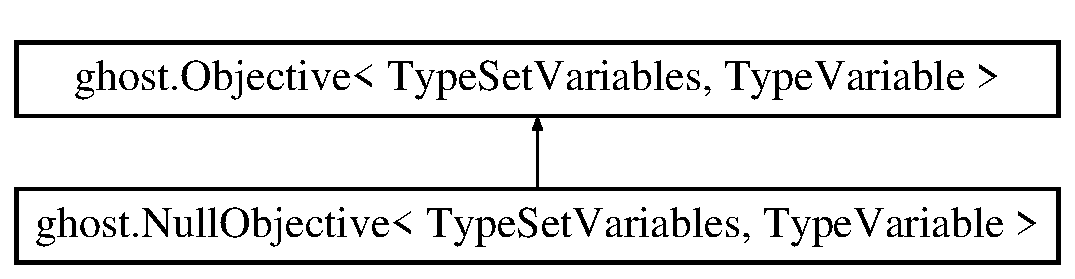
\includegraphics[height=2.000000cm]{classghost_1_1NullObjective_3_01TypeSetVariables_00_01TypeVariable_01_4}
\end{center}
\end{figure}
\subsection*{Public Member Functions}
\begin{DoxyCompactItemize}
\item 
\hypertarget{classghost_1_1NullObjective_3_01TypeSetVariables_00_01TypeVariable_01_4_a644e5a014d52e576153c362d3c9de538}{override double {\bfseries Cost} (Type\-Set\-Variables variables)}\label{classghost_1_1NullObjective_3_01TypeSetVariables_00_01TypeVariable_01_4_a644e5a014d52e576153c362d3c9de538}

\end{DoxyCompactItemize}
\subsection*{Additional Inherited Members}


The documentation for this class was generated from the following file\-:\begin{DoxyCompactItemize}
\item 
Ghost/src/Objective.\-cs\end{DoxyCompactItemize}

\hypertarget{classghost_1_1Objective_3_01TypeSetVariables_00_01TypeVariable_01_4}{\section{ghost.\-Objective$<$ Type\-Set\-Variables, Type\-Variable $>$ Class Template Reference}
\label{classghost_1_1Objective_3_01TypeSetVariables_00_01TypeVariable_01_4}\index{ghost.\-Objective$<$ Type\-Set\-Variables, Type\-Variable $>$@{ghost.\-Objective$<$ Type\-Set\-Variables, Type\-Variable $>$}}
}
Inheritance diagram for ghost.\-Objective$<$ Type\-Set\-Variables, Type\-Variable $>$\-:\begin{figure}[H]
\begin{center}
\leavevmode
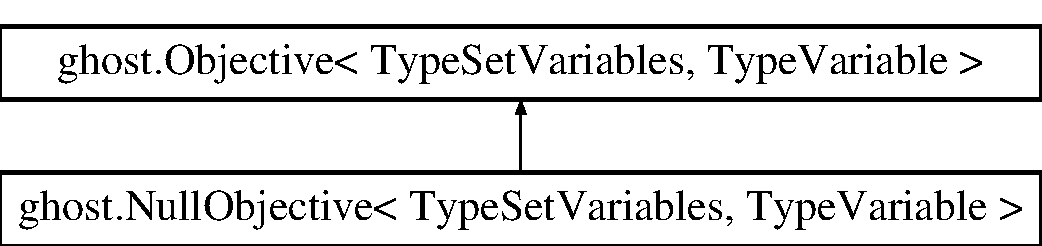
\includegraphics[height=2.000000cm]{classghost_1_1Objective_3_01TypeSetVariables_00_01TypeVariable_01_4}
\end{center}
\end{figure}
\subsection*{Public Member Functions}
\begin{DoxyCompactItemize}
\item 
\hypertarget{classghost_1_1Objective_3_01TypeSetVariables_00_01TypeVariable_01_4_a0c12ac631a5d034441c8192597b018e3}{abstract double {\bfseries Cost} (Type\-Set\-Variables variables)}\label{classghost_1_1Objective_3_01TypeSetVariables_00_01TypeVariable_01_4_a0c12ac631a5d034441c8192597b018e3}

\item 
\hypertarget{classghost_1_1Objective_3_01TypeSetVariables_00_01TypeVariable_01_4_a64c523482c82c5fcbffa31a0a57aeb48}{virtual int {\bfseries Heuristic\-Variable} (List$<$ int $>$ indexes, Type\-Set\-Variables variables)}\label{classghost_1_1Objective_3_01TypeSetVariables_00_01TypeVariable_01_4_a64c523482c82c5fcbffa31a0a57aeb48}

\item 
\hypertarget{classghost_1_1Objective_3_01TypeSetVariables_00_01TypeVariable_01_4_ababf3021752413ec655afb785d140627}{virtual int {\bfseries Heuristic\-Value} (List$<$ int $>$ values\-Index, int variable\-Index, Type\-Set\-Variables variables)}\label{classghost_1_1Objective_3_01TypeSetVariables_00_01TypeVariable_01_4_ababf3021752413ec655afb785d140627}

\item 
\hypertarget{classghost_1_1Objective_3_01TypeSetVariables_00_01TypeVariable_01_4_acc3900b803f6e1ada95c1e4b5a8f0857}{virtual double {\bfseries Postprocess\-Satisfaction} (Type\-Set\-Variables variables, ref double best\-Cost, List$<$ int $>$ solution, double sat\-Timeout)}\label{classghost_1_1Objective_3_01TypeSetVariables_00_01TypeVariable_01_4_acc3900b803f6e1ada95c1e4b5a8f0857}

\item 
\hypertarget{classghost_1_1Objective_3_01TypeSetVariables_00_01TypeVariable_01_4_a699f37da4873761f4b3c9721f140c56a}{virtual double {\bfseries Postprocess\-Optimization} (Type\-Set\-Variables variables, ref double best\-Cost, double opt\-Timeout)}\label{classghost_1_1Objective_3_01TypeSetVariables_00_01TypeVariable_01_4_a699f37da4873761f4b3c9721f140c56a}

\end{DoxyCompactItemize}
\subsection*{Protected Member Functions}
\begin{DoxyCompactItemize}
\item 
\hypertarget{classghost_1_1Objective_3_01TypeSetVariables_00_01TypeVariable_01_4_a036b0e1d3b3678f38f5080a1a32e27f4}{{\bfseries Objective} (string name, bool permutation=false)}\label{classghost_1_1Objective_3_01TypeSetVariables_00_01TypeVariable_01_4_a036b0e1d3b3678f38f5080a1a32e27f4}

\end{DoxyCompactItemize}
\subsection*{Properties}
\begin{DoxyCompactItemize}
\item 
\hypertarget{classghost_1_1Objective_3_01TypeSetVariables_00_01TypeVariable_01_4_a7613aecfe171eb9aa6f3b77ccdbe49be}{string {\bfseries Name}\hspace{0.3cm}{\ttfamily  \mbox{[}get, set\mbox{]}}}\label{classghost_1_1Objective_3_01TypeSetVariables_00_01TypeVariable_01_4_a7613aecfe171eb9aa6f3b77ccdbe49be}

\item 
\hypertarget{classghost_1_1Objective_3_01TypeSetVariables_00_01TypeVariable_01_4_ae27cf3769e4705f74e22a32604982375}{bool {\bfseries Is\-Permutation}\hspace{0.3cm}{\ttfamily  \mbox{[}get, set\mbox{]}}}\label{classghost_1_1Objective_3_01TypeSetVariables_00_01TypeVariable_01_4_ae27cf3769e4705f74e22a32604982375}

\item 
\hypertarget{classghost_1_1Objective_3_01TypeSetVariables_00_01TypeVariable_01_4_ad1ab2a8ba444cebdf8a9e7ee692731b4}{Random {\bfseries Random}\hspace{0.3cm}{\ttfamily  \mbox{[}get, set\mbox{]}}}\label{classghost_1_1Objective_3_01TypeSetVariables_00_01TypeVariable_01_4_ad1ab2a8ba444cebdf8a9e7ee692731b4}

\end{DoxyCompactItemize}


The documentation for this class was generated from the following file\-:\begin{DoxyCompactItemize}
\item 
Ghost/src/Objective.\-cs\end{DoxyCompactItemize}

\hypertarget{classghost_1_1SetVariables_3_01TypeVariable_01_4}{\section{ghost.\-Set\-Variables$<$ Type\-Variable $>$ Class Template Reference}
\label{classghost_1_1SetVariables_3_01TypeVariable_01_4}\index{ghost.\-Set\-Variables$<$ Type\-Variable $>$@{ghost.\-Set\-Variables$<$ Type\-Variable $>$}}
}
\subsection*{Public Member Functions}
\begin{DoxyCompactItemize}
\item 
\hypertarget{classghost_1_1SetVariables_3_01TypeVariable_01_4_aa4d6976b36cca380b1581584047f7ca1}{{\bfseries Set\-Variables} (List$<$ Type\-Variable $>$ variables)}\label{classghost_1_1SetVariables_3_01TypeVariable_01_4_aa4d6976b36cca380b1581584047f7ca1}

\item 
\hypertarget{classghost_1_1SetVariables_3_01TypeVariable_01_4_a1d8990709787aadaf0e5180aa0cf7414}{void {\bfseries Random\-Initialization} ()}\label{classghost_1_1SetVariables_3_01TypeVariable_01_4_a1d8990709787aadaf0e5180aa0cf7414}

\item 
\hypertarget{classghost_1_1SetVariables_3_01TypeVariable_01_4_ab56b789dea78a2a6b831b567efc3b3d0}{int {\bfseries Get\-Number\-Variables} ()}\label{classghost_1_1SetVariables_3_01TypeVariable_01_4_ab56b789dea78a2a6b831b567efc3b3d0}

\item 
\hypertarget{classghost_1_1SetVariables_3_01TypeVariable_01_4_a2473f5c049d319412e81b440493d67e8}{int {\bfseries Get\-Size\-All\-Domains} ()}\label{classghost_1_1SetVariables_3_01TypeVariable_01_4_a2473f5c049d319412e81b440493d67e8}

\item 
\hypertarget{classghost_1_1SetVariables_3_01TypeVariable_01_4_a2f8e4117bea08d33024b3da31baf5a09}{int {\bfseries Get\-Index} (Type\-Variable variable)}\label{classghost_1_1SetVariables_3_01TypeVariable_01_4_a2f8e4117bea08d33024b3da31baf5a09}

\item 
\hypertarget{classghost_1_1SetVariables_3_01TypeVariable_01_4_a3554ef33a14c339391af02d0a04723b0}{bool {\bfseries Is\-In\-Set} (Type\-Variable variable)}\label{classghost_1_1SetVariables_3_01TypeVariable_01_4_a3554ef33a14c339391af02d0a04723b0}

\item 
\hypertarget{classghost_1_1SetVariables_3_01TypeVariable_01_4_a3b1af09bf19f7d39d57b127da543133a}{void {\bfseries Swap} (int index1, int index2)}\label{classghost_1_1SetVariables_3_01TypeVariable_01_4_a3b1af09bf19f7d39d57b127da543133a}

\item 
\hypertarget{classghost_1_1SetVariables_3_01TypeVariable_01_4_ad4382f298c7b54fb6cb03a673051700f}{virtual void {\bfseries Reset\-Domain} (int index)}\label{classghost_1_1SetVariables_3_01TypeVariable_01_4_ad4382f298c7b54fb6cb03a673051700f}

\item 
\hypertarget{classghost_1_1SetVariables_3_01TypeVariable_01_4_a2a1663cb1d1728506ed0c28a8701b18e}{virtual void {\bfseries Reset\-All\-Domains} ()}\label{classghost_1_1SetVariables_3_01TypeVariable_01_4_a2a1663cb1d1728506ed0c28a8701b18e}

\item 
\hypertarget{classghost_1_1SetVariables_3_01TypeVariable_01_4_a4e762f134c7e90bf3aeb8f26d976dbe6}{virtual void {\bfseries Shift\-Value} (int index)}\label{classghost_1_1SetVariables_3_01TypeVariable_01_4_a4e762f134c7e90bf3aeb8f26d976dbe6}

\item 
\hypertarget{classghost_1_1SetVariables_3_01TypeVariable_01_4_a67a402616d76235dd929099ebbe321a9}{virtual void {\bfseries Unshift\-Value} (int index)}\label{classghost_1_1SetVariables_3_01TypeVariable_01_4_a67a402616d76235dd929099ebbe321a9}

\item 
\hypertarget{classghost_1_1SetVariables_3_01TypeVariable_01_4_a4a5330430dfd94a46a718e28a0355d91}{virtual int {\bfseries Get\-Value} (int index)}\label{classghost_1_1SetVariables_3_01TypeVariable_01_4_a4a5330430dfd94a46a718e28a0355d91}

\item 
\hypertarget{classghost_1_1SetVariables_3_01TypeVariable_01_4_a6f4f72d36727cf96522ed6e5635b5c27}{virtual void {\bfseries Set\-Value} (int index, int value)}\label{classghost_1_1SetVariables_3_01TypeVariable_01_4_a6f4f72d36727cf96522ed6e5635b5c27}

\item 
\hypertarget{classghost_1_1SetVariables_3_01TypeVariable_01_4_ad382b5c9045b7f5d5bc1baf2b8121bb4}{virtual List$<$ int $>$ {\bfseries Possible\-Values} (int index)}\label{classghost_1_1SetVariables_3_01TypeVariable_01_4_ad382b5c9045b7f5d5bc1baf2b8121bb4}

\item 
\hypertarget{classghost_1_1SetVariables_3_01TypeVariable_01_4_adea50d515383d6c0252d36a164213d83}{string {\bfseries Name} (int index)}\label{classghost_1_1SetVariables_3_01TypeVariable_01_4_adea50d515383d6c0252d36a164213d83}

\item 
\hypertarget{classghost_1_1SetVariables_3_01TypeVariable_01_4_a7f32c243dd4c5b434c2b3d51c8b37e5e}{string {\bfseries Full\-Name} (int index)}\label{classghost_1_1SetVariables_3_01TypeVariable_01_4_a7f32c243dd4c5b434c2b3d51c8b37e5e}

\item 
\hypertarget{classghost_1_1SetVariables_3_01TypeVariable_01_4_ab9627fb96652fc476da1a0d04ebdc815}{\hyperlink{classghost_1_1Domain}{Domain} {\bfseries Domain} (int index)}\label{classghost_1_1SetVariables_3_01TypeVariable_01_4_ab9627fb96652fc476da1a0d04ebdc815}

\item 
\hypertarget{classghost_1_1SetVariables_3_01TypeVariable_01_4_ac254fd0d11c3effcaff7689d9954062b}{virtual void {\bfseries Print} ()}\label{classghost_1_1SetVariables_3_01TypeVariable_01_4_ac254fd0d11c3effcaff7689d9954062b}

\end{DoxyCompactItemize}
\subsection*{Properties}
\begin{DoxyCompactItemize}
\item 
\hypertarget{classghost_1_1SetVariables_3_01TypeVariable_01_4_a1aa6a24ebcf2782dbd09e186e5c000d8}{List$<$ Type\-Variable $>$ {\bfseries Variables}\hspace{0.3cm}{\ttfamily  \mbox{[}get, set\mbox{]}}}\label{classghost_1_1SetVariables_3_01TypeVariable_01_4_a1aa6a24ebcf2782dbd09e186e5c000d8}

\end{DoxyCompactItemize}


The documentation for this class was generated from the following file\-:\begin{DoxyCompactItemize}
\item 
Ghost/src/Set\-Variables.\-cs\end{DoxyCompactItemize}

\hypertarget{classghost_1_1Solver_3_01TypeVariable_00_01TypeSetVariables_00_01TypeConstraint_01_4}{\section{ghost.\-Solver$<$ Type\-Variable, Type\-Set\-Variables, Type\-Constraint $>$ Class Template Reference}
\label{classghost_1_1Solver_3_01TypeVariable_00_01TypeSetVariables_00_01TypeConstraint_01_4}\index{ghost.\-Solver$<$ Type\-Variable, Type\-Set\-Variables, Type\-Constraint $>$@{ghost.\-Solver$<$ Type\-Variable, Type\-Set\-Variables, Type\-Constraint $>$}}
}
\subsection*{Public Member Functions}
\begin{DoxyCompactItemize}
\item 
\hypertarget{classghost_1_1Solver_3_01TypeVariable_00_01TypeSetVariables_00_01TypeConstraint_01_4_a09dc7b1660980591f5f60619420d44ca}{{\bfseries Solver} (Type\-Set\-Variables vec\-Variables, List$<$ Type\-Constraint $>$ vec\-Constraints, Objective$<$ Type\-Set\-Variables, Type\-Variable $>$ obj=null)}\label{classghost_1_1Solver_3_01TypeVariable_00_01TypeSetVariables_00_01TypeConstraint_01_4_a09dc7b1660980591f5f60619420d44ca}

\item 
\hypertarget{classghost_1_1Solver_3_01TypeVariable_00_01TypeSetVariables_00_01TypeConstraint_01_4_a83d8d09f96d154da1d928288a36ea0e2}{{\bfseries Solver} (Type\-Set\-Variables vec\-Variables, List$<$ Type\-Constraint $>$ vec\-Constraints, Objective$<$ Type\-Set\-Variables, Type\-Variable $>$ obj, int loops)}\label{classghost_1_1Solver_3_01TypeVariable_00_01TypeSetVariables_00_01TypeConstraint_01_4_a83d8d09f96d154da1d928288a36ea0e2}

\item 
\hypertarget{classghost_1_1Solver_3_01TypeVariable_00_01TypeSetVariables_00_01TypeConstraint_01_4_a9ad3017bd3ff361497491766214fdacd}{double {\bfseries solve} (double sat\-Timeout, double opt\-Timeout=0, bool do\-Random\-Initialization=true)}\label{classghost_1_1Solver_3_01TypeVariable_00_01TypeSetVariables_00_01TypeConstraint_01_4_a9ad3017bd3ff361497491766214fdacd}

\end{DoxyCompactItemize}


The documentation for this class was generated from the following file\-:\begin{DoxyCompactItemize}
\item 
Ghost/src/Solver.\-cs\end{DoxyCompactItemize}

\hypertarget{classghost_1_1Variable}{\section{ghost.\-Variable Class Reference}
\label{classghost_1_1Variable}\index{ghost.\-Variable@{ghost.\-Variable}}
}
\subsection*{Public Member Functions}
\begin{DoxyCompactItemize}
\item 
void \hyperlink{classghost_1_1Variable_abeb22408704798a971c6081a27d02512}{Reset\-Domain} ()
\item 
void \hyperlink{classghost_1_1Variable_a96bc6a1826d8217cbdcbd77c6acd6107}{Shift\-Value} ()
\item 
void \hyperlink{classghost_1_1Variable_a94aabd7fa16ea55c30df67bc9b179300}{Unshift\-Value} ()
\item 
int \hyperlink{classghost_1_1Variable_a13ab07f2257acacecaa3afe9910cd5d8}{Get\-Value} ()
\item 
void \hyperlink{classghost_1_1Variable_a3b1051f1ae8e722e8733a64ee124486d}{Set\-Value} (int value)
\item 
List$<$ int $>$ \hyperlink{classghost_1_1Variable_a4f3523cf1d3b5a8dc6db9f4661bea285}{Possible\-Values} ()
\end{DoxyCompactItemize}
\subsection*{Protected Member Functions}
\begin{DoxyCompactItemize}
\item 
\hyperlink{classghost_1_1Variable_a6f8316e07669cd8bf41257756bca929f}{Variable} (string name, string full\-Name)
\item 
\hyperlink{classghost_1_1Variable_ac314e16271744bd04e8fdfa105b2afde}{Variable} (string name, string full\-Name, \hyperlink{classghost_1_1Domain}{Domain} domain, int value)
\end{DoxyCompactItemize}
\subsection*{Properties}
\begin{DoxyCompactItemize}
\item 
string \hyperlink{classghost_1_1Variable_a1dba3848c7675d086eecad078178e4d9}{Name}\hspace{0.3cm}{\ttfamily  \mbox{[}get, set\mbox{]}}
\item 
string \hyperlink{classghost_1_1Variable_af20c2f01306cba69f36d32babb703c1d}{Full\-Name}\hspace{0.3cm}{\ttfamily  \mbox{[}get, set\mbox{]}}
\item 
\hyperlink{classghost_1_1Domain}{Domain} \hyperlink{classghost_1_1Variable_aae96e8a30ff2f44dc115a0b51e136e92}{Domain}\hspace{0.3cm}{\ttfamily  \mbox{[}get, set\mbox{]}}
\item 
int \hyperlink{classghost_1_1Variable_a4fa08b5d46a4559d345d4752e7a790d2}{Index\-Domain}\hspace{0.3cm}{\ttfamily  \mbox{[}get, set\mbox{]}}
\end{DoxyCompactItemize}


\subsection{Detailed Description}
\hyperlink{classghost_1_1Variable}{Variable} is the abstract class giving a generic interface of variables. A variable is characterised by a name, a long name (called full name), a \hyperlink{classghost_1_1Domain}{Domain} and its current value (actually, an iterator on its \hyperlink{classghost_1_1Domain}{Domain}). 

\subsection{Constructor \& Destructor Documentation}
\hypertarget{classghost_1_1Variable_a6f8316e07669cd8bf41257756bca929f}{\index{ghost\-::\-Variable@{ghost\-::\-Variable}!Variable@{Variable}}
\index{Variable@{Variable}!ghost::Variable@{ghost\-::\-Variable}}
\subsubsection[{Variable}]{\setlength{\rightskip}{0pt plus 5cm}ghost.\-Variable.\-Variable (
\begin{DoxyParamCaption}
\item[{string}]{name, }
\item[{string}]{full\-Name}
\end{DoxyParamCaption}
)\hspace{0.3cm}{\ttfamily [inline]}, {\ttfamily [protected]}}}\label{classghost_1_1Variable_a6f8316e07669cd8bf41257756bca929f}
Constructor where the domain will be instanciated by default. \hypertarget{classghost_1_1Variable_ac314e16271744bd04e8fdfa105b2afde}{\index{ghost\-::\-Variable@{ghost\-::\-Variable}!Variable@{Variable}}
\index{Variable@{Variable}!ghost::Variable@{ghost\-::\-Variable}}
\subsubsection[{Variable}]{\setlength{\rightskip}{0pt plus 5cm}ghost.\-Variable.\-Variable (
\begin{DoxyParamCaption}
\item[{string}]{name, }
\item[{string}]{full\-Name, }
\item[{{\bf Domain}}]{domain, }
\item[{int}]{value}
\end{DoxyParamCaption}
)\hspace{0.3cm}{\ttfamily [inline]}, {\ttfamily [protected]}}}\label{classghost_1_1Variable_ac314e16271744bd04e8fdfa105b2afde}
Regular constructor. The domain is cloned or instanciated if null. The domain iterator is assigned to the index of value in \hyperlink{classghost_1_1Domain}{Domain}, or to -\/42 if the \hyperlink{classghost_1_1Domain}{Domain} has not been initialized. \begin{DoxySeeAlso}{See Also}
\hyperlink{classghost_1_1Domain_a19610b0d083f6a47eeb867fbcf8c0522}{Domain.\-Is\-Initialized()} 
\end{DoxySeeAlso}


\subsection{Member Function Documentation}
\hypertarget{classghost_1_1Variable_a13ab07f2257acacecaa3afe9910cd5d8}{\index{ghost\-::\-Variable@{ghost\-::\-Variable}!Get\-Value@{Get\-Value}}
\index{Get\-Value@{Get\-Value}!ghost::Variable@{ghost\-::\-Variable}}
\subsubsection[{Get\-Value}]{\setlength{\rightskip}{0pt plus 5cm}int ghost.\-Variable.\-Get\-Value (
\begin{DoxyParamCaption}
{}
\end{DoxyParamCaption}
)\hspace{0.3cm}{\ttfamily [inline]}}}\label{classghost_1_1Variable_a13ab07f2257acacecaa3afe9910cd5d8}
To knwo the current variable value. \begin{DoxyReturn}{Returns}
An integer corresponding to the variable's current value. 
\end{DoxyReturn}
\hypertarget{classghost_1_1Variable_a4f3523cf1d3b5a8dc6db9f4661bea285}{\index{ghost\-::\-Variable@{ghost\-::\-Variable}!Possible\-Values@{Possible\-Values}}
\index{Possible\-Values@{Possible\-Values}!ghost::Variable@{ghost\-::\-Variable}}
\subsubsection[{Possible\-Values}]{\setlength{\rightskip}{0pt plus 5cm}List$<$int$>$ ghost.\-Variable.\-Possible\-Values (
\begin{DoxyParamCaption}
{}
\end{DoxyParamCaption}
)\hspace{0.3cm}{\ttfamily [inline]}}}\label{classghost_1_1Variable_a4f3523cf1d3b5a8dc6db9f4661bea285}
To know what values are in the current domain. \begin{DoxyReturn}{Returns}
a List$<$int$>$ of values belonging to the variable domain. 
\end{DoxyReturn}
\hypertarget{classghost_1_1Variable_abeb22408704798a971c6081a27d02512}{\index{ghost\-::\-Variable@{ghost\-::\-Variable}!Reset\-Domain@{Reset\-Domain}}
\index{Reset\-Domain@{Reset\-Domain}!ghost::Variable@{ghost\-::\-Variable}}
\subsubsection[{Reset\-Domain}]{\setlength{\rightskip}{0pt plus 5cm}void ghost.\-Variable.\-Reset\-Domain (
\begin{DoxyParamCaption}
{}
\end{DoxyParamCaption}
)\hspace{0.3cm}{\ttfamily [inline]}}}\label{classghost_1_1Variable_abeb22408704798a971c6081a27d02512}
Reset the variable's domain to its initial values. \begin{DoxySeeAlso}{See Also}
\hyperlink{classghost_1_1Domain_a732f5cc39dba50b1abbfc37664a3bbb7}{Domain.\-Reset\-To\-Initial()} 
\end{DoxySeeAlso}
\hypertarget{classghost_1_1Variable_a3b1051f1ae8e722e8733a64ee124486d}{\index{ghost\-::\-Variable@{ghost\-::\-Variable}!Set\-Value@{Set\-Value}}
\index{Set\-Value@{Set\-Value}!ghost::Variable@{ghost\-::\-Variable}}
\subsubsection[{Set\-Value}]{\setlength{\rightskip}{0pt plus 5cm}void ghost.\-Variable.\-Set\-Value (
\begin{DoxyParamCaption}
\item[{int}]{value}
\end{DoxyParamCaption}
)\hspace{0.3cm}{\ttfamily [inline]}}}\label{classghost_1_1Variable_a3b1051f1ae8e722e8733a64ee124486d}
Set the current value. \hypertarget{classghost_1_1Variable_a96bc6a1826d8217cbdcbd77c6acd6107}{\index{ghost\-::\-Variable@{ghost\-::\-Variable}!Shift\-Value@{Shift\-Value}}
\index{Shift\-Value@{Shift\-Value}!ghost::Variable@{ghost\-::\-Variable}}
\subsubsection[{Shift\-Value}]{\setlength{\rightskip}{0pt plus 5cm}void ghost.\-Variable.\-Shift\-Value (
\begin{DoxyParamCaption}
{}
\end{DoxyParamCaption}
)\hspace{0.3cm}{\ttfamily [inline]}}}\label{classghost_1_1Variable_a96bc6a1826d8217cbdcbd77c6acd6107}
Set the current value to the next value in the domain, or to the first one if we reach the domain upper bound. \hypertarget{classghost_1_1Variable_a94aabd7fa16ea55c30df67bc9b179300}{\index{ghost\-::\-Variable@{ghost\-::\-Variable}!Unshift\-Value@{Unshift\-Value}}
\index{Unshift\-Value@{Unshift\-Value}!ghost::Variable@{ghost\-::\-Variable}}
\subsubsection[{Unshift\-Value}]{\setlength{\rightskip}{0pt plus 5cm}void ghost.\-Variable.\-Unshift\-Value (
\begin{DoxyParamCaption}
{}
\end{DoxyParamCaption}
)\hspace{0.3cm}{\ttfamily [inline]}}}\label{classghost_1_1Variable_a94aabd7fa16ea55c30df67bc9b179300}
Set the current value to the previous value in the domain, or to the last one if we reach the domain lower bound. 

\subsection{Property Documentation}
\hypertarget{classghost_1_1Variable_aae96e8a30ff2f44dc115a0b51e136e92}{\index{ghost\-::\-Variable@{ghost\-::\-Variable}!Domain@{Domain}}
\index{Domain@{Domain}!ghost::Variable@{ghost\-::\-Variable}}
\subsubsection[{Domain}]{\setlength{\rightskip}{0pt plus 5cm}{\bf Domain} ghost.\-Variable.\-Domain\hspace{0.3cm}{\ttfamily [get]}, {\ttfamily [set]}}}\label{classghost_1_1Variable_aae96e8a30ff2f44dc115a0b51e136e92}
The \hyperlink{classghost_1_1Domain}{Domain}, ie, the list of possible variable values \hypertarget{classghost_1_1Variable_af20c2f01306cba69f36d32babb703c1d}{\index{ghost\-::\-Variable@{ghost\-::\-Variable}!Full\-Name@{Full\-Name}}
\index{Full\-Name@{Full\-Name}!ghost::Variable@{ghost\-::\-Variable}}
\subsubsection[{Full\-Name}]{\setlength{\rightskip}{0pt plus 5cm}string ghost.\-Variable.\-Full\-Name\hspace{0.3cm}{\ttfamily [get]}, {\ttfamily [set]}}}\label{classghost_1_1Variable_af20c2f01306cba69f36d32babb703c1d}
Full\-Name is the long name of the variable. For instance, 'building'. \hypertarget{classghost_1_1Variable_a4fa08b5d46a4559d345d4752e7a790d2}{\index{ghost\-::\-Variable@{ghost\-::\-Variable}!Index\-Domain@{Index\-Domain}}
\index{Index\-Domain@{Index\-Domain}!ghost::Variable@{ghost\-::\-Variable}}
\subsubsection[{Index\-Domain}]{\setlength{\rightskip}{0pt plus 5cm}int ghost.\-Variable.\-Index\-Domain\hspace{0.3cm}{\ttfamily [get]}, {\ttfamily [set]}, {\ttfamily [protected]}}}\label{classghost_1_1Variable_a4fa08b5d46a4559d345d4752e7a790d2}
A variable does not contain its current value directly, but the domain index of its current value. This acts like on iterator on the domain \hypertarget{classghost_1_1Variable_a1dba3848c7675d086eecad078178e4d9}{\index{ghost\-::\-Variable@{ghost\-::\-Variable}!Name@{Name}}
\index{Name@{Name}!ghost::Variable@{ghost\-::\-Variable}}
\subsubsection[{Name}]{\setlength{\rightskip}{0pt plus 5cm}string ghost.\-Variable.\-Name\hspace{0.3cm}{\ttfamily [get]}, {\ttfamily [set]}}}\label{classghost_1_1Variable_a1dba3848c7675d086eecad078178e4d9}
Name is the short name of the variable. For instance, 'b'. 

The documentation for this class was generated from the following file\-:\begin{DoxyCompactItemize}
\item 
Ghost/src/Variable.\-cs\end{DoxyCompactItemize}

%--- End generated contents ---

% Index
\newpage
\phantomsection
\addcontentsline{toc}{chapter}{Index}
\printindex

\end{document}
